\documentclass[11pt,a4paper]{article}
\usepackage[czech]{babel}
\usepackage[utf8]{inputenc}
\usepackage{times}
\usepackage{url}
\usepackage[textwidth=15.2cm,textheight=23cm]{geometry}
\usepackage{xcolor}

\usepackage{graphicx}

%\usepackage{fancyvrb}
%\DefineVerbatimEnvironment{verbatim}{Verbatim}{}

\usepackage[bf]{caption}

\usepackage[hyperindex,
  plainpages=false,
  pdftex,
  colorlinks,
  pdfborder={0 0 0},
  pdfpagelabels]{hyperref}

\pdfcompresslevel=9

\newcommand{\myincludegraphics}[4]{
  \begin{figure}[!h]
  \centering
  \includegraphics[#1]{#2}
  \caption{#3.} \label{#4}
  \end{figure}
}

% titulní stránka a obsah
\newcommand{\titlepageandcontents}{
  \begin{titlepage}

\vspace*{1cm}

\begin{figure}
  \centering
  
\includegraphics[height=6cm]{images/fit.pdf}
\end{figure}

\vspace*{5mm}

\begin{center}
\begin{Large}
Projekt do předmětu PDB -- Pokročilé databázové systémy
\end{Large}
\end{center}

\vspace*{5mm}

\begin{center}
\begin{Huge}
Prostorové, multimediální a temporální databáze\\
\end{Huge}
\end{center}

\vspace*{1cm}

\begin{center}
\begin{Large}
\today
\end{Large}
\end{center}

\vfill

\begin{flushleft}
\begin{large}
\begin{tabular}{ll}

\bf Řešitelé:\hspace{3mm} & Tomáš Mikulica (\verb_xmikul45@stud.fit.vutbr.cz_) \\
& Miroslav Paulík (\verb_xpauli00@stud.fit.vutbr.cz_) \\
& Pavel Gajdoš (\verb xgajdo13@stud.fit.vutbr.cz) \\
& Fakulta Informačních Technologií \\
& Vysoké Učení Technické v~Brně

\end{tabular}
\end{large}
\end{flushleft}

\end{titlepage}

% vim:set ft=tex expandtab enc=utf8:


  \pagestyle{plain}
  \pagenumbering{roman}
  \setcounter{page}{1}
  %\tableofcontents

  \newpage
  \pagestyle{plain}
  \pagenumbering{arabic}
  \setcounter{page}{1}
}

\def\uv#1{\iflanguage{english}{``#1''}%
                              {\quotedblbase #1\textquotedblleft}}%

\newcommand\todo[1]{\textcolor{red}{[[TODO: #1]]}}
\newcommand\blindtextGray{\textcolor{gray}{\blindtext}}
\newcommand\comment[1]{}

% vim:set ft=tex expandtab enc=utf8:

\usepackage{amsmath}
\usepackage{moreverb}
\newcommand\mycomment[1]{}


\begin{document} \sloppy
\titlepageandcontents

\section{Spuštení a nastavení aplikace}
Pro spuštení projektu stačí otevřít obsah rozbaleného archivu jako projekt ve vývojovém studiu \emph{NetBeans}\footnote{\url{https://netbeans.org/}}.

\section{Přihlašovací obrazovka a naplnění vzorové databáze}\label{sec1}
Po spuštění aplikace se jako první záložka aplikace objeví administrace. Na této kartě je možné:
\begin{enumerate}
 \item přihlásit se -- po vyplění údajů a stisku tlačítka 1 z obrázku \ref{admin}
 \item přihlásit se jako host -- v případě, že máme dostupný konfigurační soubor (více viz kapitola \ref{conf}), a stiskem tlačítka 2
 \item resetovat databázi do původního stavu -- stiskem tlačítka 3
 \end{enumerate}
 Možnost resetovat databázi je dostupná až po přihlášení uživatele.

%---obrazek
\begin{figure}[h!]
\begin{center}
\scalebox{1.0}{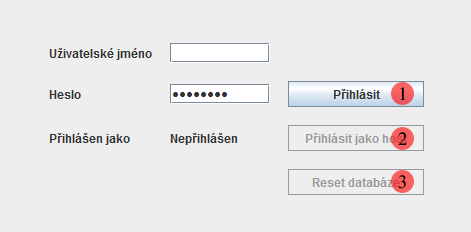
\includegraphics{images/login.png}}
\caption{Obrazovka administrace.}
\label{admin}
\end{center}
\end{figure}
%---konec obrazek

 \subsection{Konfigurační soubor}\label{conf}
 Aby se nemuseli pro každé přihlášení znovu vyplňovat přihlašovací údaje, je v aplikaci možnost automatického připojení skrze údaje uložené v konfiguračním souboru. Ten je ve tvaru:
 \begin{center}
\begin{boxedverbatim}
DB.LOGIN=login
DB.PASSWORD=password

DB.HOST=hostaddress
DB.PORT=port
DB.SID=dbname
\end{boxedverbatim}
\end{center}
Tento soubor se musí jmenovat \texttt{config.local.properties} a musí být v adresáři \verb;PDB-projekt\src\cz\vutbr\fit\pdb\config;. V případě existence tohoto souboru se pokusí aplikace po spuštení připojit k databázi automaticky, aniž by bylo nutné na něco klikat.

\subsection{Přístupové údaje k databázím}

\begin{center}
  \begin{tabular}{ | c || c | c |}
  	\hline
  	Jméno a příjmení & login & heslo\\
    \hline\hline
    Tomáš Mikulica & xmikul45 & 3mycjfdc \\ \hline
    Miroslav Paulík & xpauli00 & pa2mx4qu \\ \hline
    Pavel Gajdoš & xgajdo13 & 4q5ro7dz \\
    \hline
  \end{tabular}
\end{center}

\section{Ovládání aplikace}
Aplikace je rozdělena do několika záložek: 
\begin{itemize}
\item \textbf{Administrace} -- popsána v sekci \ref{sec1}
\item \textbf{Služby} -- V této záložce je zobrazena mapa areálu. Při kliknutí (pokud je aktivní zezelená) na objekt je možné tento objekt zarezervovat pro ubytované hosty. Rezervuje se na hodinu a je možné zvolit i konkrétní datum. Rezervace se potvrdí stiskem tlačítka ``Uložit změny''.

\item \textbf{Areál} -- V této záložce je možné areál upravovat - lze přidávat nebo mazat geometrické entity s vlastními uživatelskými názvy. Lze vytvářet mnohoúhelník, kruh, křivku a bod. Dále zde lze provádět operace nad prostorovými daty. Po vytvoření nějaké entity je třeba změny potvrdit kliknutím na {\em Uložit změny}. Neuložené změny lze zrušit kliknutím na tlačítko {\em Zrušit}. Bližší popis operace si zaslouží operace {\em SPOJIT}. Tato operace vyhledává všechny vzájemně se překrývající entity a tyto entity spojuje do jedné. 


\item \textbf{Fotografie} -- V této záložce je možné si prohlédnout uložené fotografie automobilů zákazníků a případně vyhledávat podle obsahu fotografie. Dále je zde možné s fotografiemi otáčet a mazat je. Pro jakoukoliv operaci (vyjma přechodu na předchozí/další fotografii) s fotografiemi je ji nutné nejdříve označit levým klikem na fotografii (projeví se zeleným orámováním fotografie).
\item \textbf{Rezervace} -- V této záložce je možné si zobrazit seznam rezervací pokojů v zadaném období, dále je možné vytvořit novou rezervaci a případně vyhlásit stav karantény.
\end{itemize}
%---obrazek
\mycomment{\begin{figure}[h!]
\begin{center}
\scalebox{0.5}{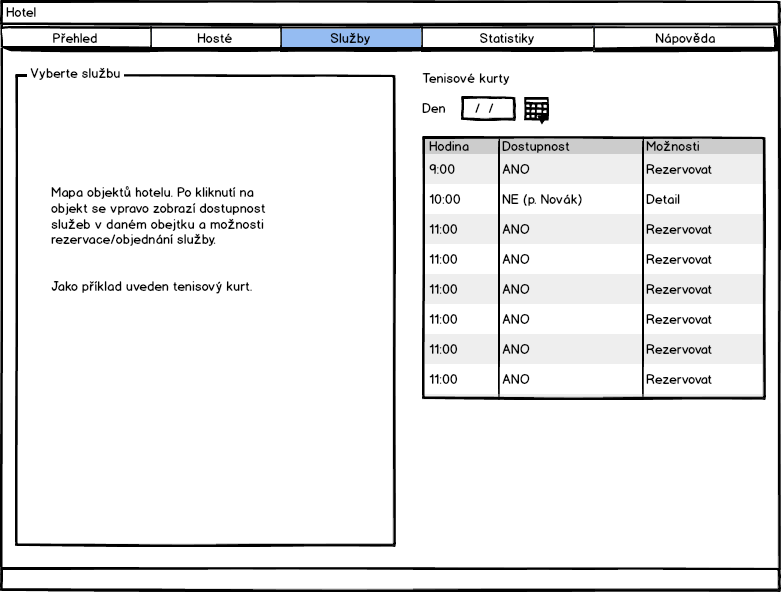
\includegraphics{images/sluzby.png}}
\caption{Obrazovka služeb.}
\label{sluzby}
\end{center}
\end{figure}}
%---konec obrazek
%---obrazek
\mycomment{\begin{figure}[h!]
\begin{center}
\scalebox{0.6}{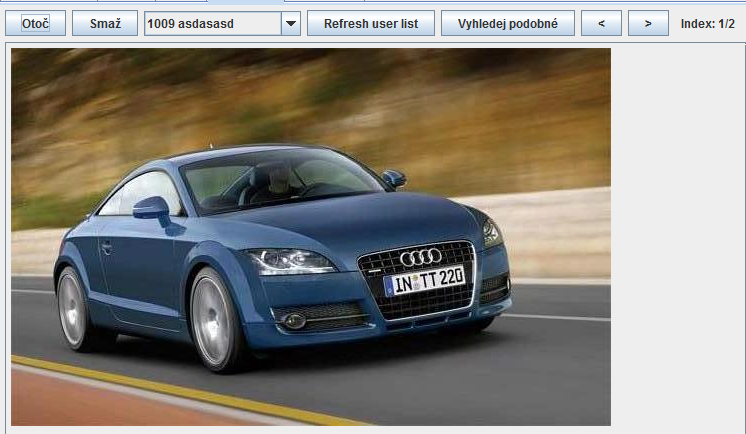
\includegraphics{images/fotografie.png}}
\caption{Obrazovka fotografií.}
\label{foto}
\end{center}
\end{figure}}
%---konec obrazek
\end{document}
